\section{A specification, and what it costs to ignore it}
\label{sec:specification}
% BUDGET: 3/4 column.  No table if space is tight -- the numbers carry it.
%
%   axis 1  denominator: covered skeleton only, or the whole ground truth
%   axis 2  fragment length: pixel count, 8-neighbour edge weights, diameter
%   axis 3  does a bridged gap split a run
%
% Crossed on \specArms{} arms x \specSeeds{} seeds, the spread is
% \specSpreadLo--\specSpreadHi{} points, against a largest honest effect of
% \specHonest{} points in the same repository.  The ranking does not survive
% the choice: Spearman \specRho{}, largest rank move \specMove{}.
%
% Then the scaling rule, which is what makes this a specification rather
% than a complaint: the spread is bounded by how much skeleton the
% prediction fails to cover, so it shrinks on easy data
% (VessMAP \txVessmapLo--\txVessmapHi{} points at \txVessmapCov\% coverage
% against STARE's \txStareLo--\txStareHi{} at \txStareCov\%).  Read backwards:
% a paper reporting ERL on easy data hides less disagreement.

\TODO{section 4 prose}
% Budget: ~300 words (3/4 column minus the specification list below).
\FILL{12-14}

\begin{figure}[t]
  \centering
  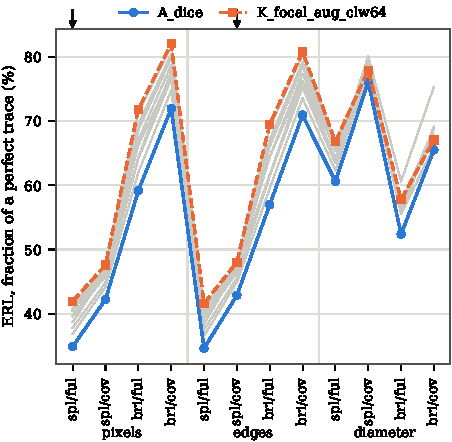
\includegraphics[width=\linewidth]{figures/fig2_conventions.pdf}
  \caption{One set of predictions on DRIVE (\specArms{} arms,
  \specSeeds{} seeds), read under each of the twelve legal cells. Grey is every
  arm; two are named. The shaded columns mark the cell the reference implementation
  computes (\texttt{split/edges/covered}) and the one this literature most often
  implements (\texttt{split/pixels/full}). Each arm spans
  \specSpreadLo--\specSpreadHi{} points without anything about the model, the
  data, the threshold or the checkpoint changing, and the arms cross: Spearman
  $\rho = \specRho$ between the two extreme cells, largest rank move
  \specMove{} of \specArms.}
  \label{fig:conventions}
\end{figure}

\begin{figure}[t]
  \centering
  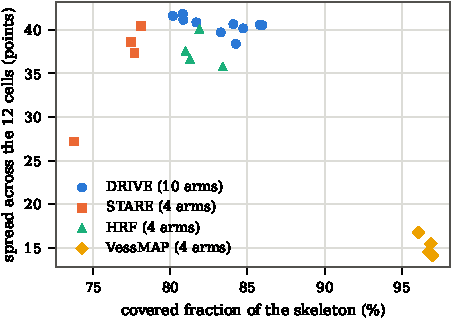
\includegraphics[width=\linewidth]{figures/fig3_coverage.pdf}
  \caption{The disagreement is not a constant. It is bounded by how much
  ground-truth skeleton the prediction fails to cover, so it collapses on easy
  data: VessMAP spans only \txVessMAPLo--\txVessMAPHi{} points at
  \txVessMAPCov\% coverage, against STARE's \txSTARELo--\txSTAREHi{} at
  \txSTARECov\%. Read backwards, a paper reporting ERL on easy data hides less
  disagreement than one on hard data.}
  \label{fig:coverage}
\end{figure}

\begin{table}[t]
  \centering
  \caption{Per-arm spread across the twelve cells, DRIVE, \specSeeds{} seeds.
  The largest honest effect any published topology loss produces in our own
  experiments, read at each arm's own dev-optimal threshold, is
  \specHonest{} points.}
  \label{tab:spread}
  \small
  % tab3_spread.tex -- GENERATED by exp/paper_figures.py. Do not edit here;
% edit the script, or the measurement it reads. Source: exp/results/heldout/erl_spec*.csv, recomputed and asserted equal to exp/results/erl_spec.txt by the selftest.
\begin{tabular}{lcccl}
\toprule
Arm & Lowest & Highest & Spread & Highest cell \\
\midrule
\texttt{H\_aug\_w64\_d5} & 38.4\% & 80.2\% & 41.8 & split/diameter/covered \\
\texttt{A\_dice} & 34.6\% & 76.2\% & 41.6 & split/diameter/covered \\
\texttt{H\_aug} & 36.5\% & 77.7\% & 41.1 & split/diameter/covered \\
\texttt{H\_aug\_clw2} & 37.5\% & 78.3\% & 40.9 & split/diameter/covered \\
\texttt{H\_aug\_clw16} & 39.3\% & 79.9\% & 40.7 & bridged/pixels/covered \\
\texttt{H\_aug\_clw64} & 41.1\% & 81.7\% & 40.6 & bridged/pixels/covered \\
\texttt{K\_focal\_aug\_clw64} & 41.6\% & 82.1\% & 40.5 & bridged/pixels/covered \\
\texttt{K\_focal\_aug\_clw32} & 40.3\% & 80.5\% & 40.2 & bridged/pixels/covered \\
\texttt{H\_aug\_clw8} & 39.4\% & 79.1\% & 39.7 & split/diameter/covered \\
\texttt{A\_dice\_clw64} & 40.1\% & 78.5\% & 38.4 & split/diameter/covered \\
\bottomrule
\end{tabular}

\end{table}


\noindent\textbf{The specification.} Report, next to every ERL number:
\begin{enumerate}
  \item the denominator, the length rule, and the splitting rule;
  \item the coverage, so the reader can convert between denominators;
  \item the amount of predicted foreground \NOTE{ERL is gameable by painting};
  \item which annotator was taken as ground truth \NOTE{5x on STARE};
  \item that the merge term does not fire, and that crossings are unpriced.
\end{enumerate}
